\documentclass{article}

\usepackage{a4wide}
\usepackage{fancyhdr}
\usepackage{graphicx}
\usepackage[ansinew]{inputenc}
\usepackage{amsmath}
\usepackage{amssymb}
\usepackage{url}
\usepackage[british]{babel}
\usepackage{listings}
\usepackage{xcolor}
\usepackage[toc, page]{appendix}
\usepackage[linesnumbered, ruled, vlined]{algorithm2e}
\usepackage{hyperref}

\definecolor{codegreen}{rgb}{0,0.6,0}
\definecolor{codegray}{rgb}{0.5,0.5,0.5}
\definecolor{codepurple}{rgb}{0.58,0,0.82}
\definecolor{backcolour}{rgb}{0.95,0.95,0.92}

\lstdefinestyle{mystyle}{
    backgroundcolor=\color{backcolour},
    commentstyle=\color{codegreen},
    keywordstyle=\color{magenta},
    numberstyle=\tiny\color{codegray},
    stringstyle=\color{codepurple},
    basicstyle=\ttfamily\footnotesize,
    breakatwhitespace=false,
    breaklines=true,
    captionpos=b,
    keepspaces=true,
    numbers=left,
    numbersep=5pt,
    showspaces=false,
    showstringspaces=false,
    showtabs=false,
    tabsize=2
}

\lstset{style=mystyle}


%%\usepackage{minted}


\title{Time-Dependent Schr{\"o}dinger Equation with Magnetic Field}
\author{Etienne Corminboeuf}
\date{\today}

\usepackage[left = 3cm, right = 3cm]{geometry}

\begin{document}

\maketitle

\tableofcontents

\section{Introduction} \label{sec:intro}
In this report we consider a spinless particle in $\mathbb{R}^d$ with mass $m \in \mathbb{R}_{\geq 0}$ and charge $e\in \mathbb{R}$ in a homogeneous magnetic field $B(t)$. We follow the notation introduced in the paper by Gradinaru and Rietmann and quickly recap the important elements. For a full derivation please consult \cite{paper_orvg}.
\subsection{Mathematic model}

In quantum mechanics, the time evolution of a particle subject to a magnetic field is governed by the Pauli equation
\begin{align} \label{eq_pauli}
  i \hbar \partial_t \Psi(x,t) &= H_P(t)\Psi(x,t) \\
  H_P(t) :&= \frac{1}{2m} \sum_{k=1}^d (p_k - e A_k(x,t))^2 + e\phi(x,t) + \tilde{V}(x,t)
\end{align}
where $\tilde{V}(x,t)$ is some external potential.
The magnetic field 2-form $dA$ associated with $B(t)$ is independent of x because of the homogeneity of $B(t)$ and we can thus rewrite the magnetic vector potential to
\begin{equation}
  A(x,t) := \frac{1}{2}B_{jk}(t)x^j \textrm{d}x^k,
\end{equation}
where $B(t)$ = $(B_{jk}(t))_{j,k = 1}^d$ is a real, skew-symmetric matrix. Using the operators
\begin{align}
  L_{jk} & := x_j p_k - x_k p_j \\
  H_B(t) & := - \sum_{j,k = 1}^d B_{jk}(t) L_{jk}
\end{align}
the Pauli-Hamiltonian takes the form
\begin{equation}
  H_P(t) = \frac{1}{2 m} \left(\hbar^{2}(-\Delta)-e \sum_{1 \leqslant j<k \leqslant d} B_{j k}(t) L_{j k} +\frac{e^{2}}{4}\|B(t) x\|_{\mathbb{R}^{d}}^{2}  \right) + e \phi(x,t) + \tilde{V}(x,t).
\end{equation}

\subsection{Numerical model}
We introduce $\epsilon ^2 := \hbar$ and redefine $t$, $x$ and $B$ to find the simplified form
\begin{equation}
  H_P(t) = -\Delta + H_B(t) + V(x,t)
\end{equation}
where $V(x,t) := \frac{1}{2m}\frac{e^{2}}{4}\|B(t) x\|_{\mathbb{R}^{d}}^{2} + e \phi(x,t) + \tilde{V}(x,t)$ can be considered to be a total effective potential.
The Schr{\"o}dinger equation
\begin{equation} \label{num_main} \tag{H}
  i \epsilon ^2 \partial_t \Psi(x, t) = H_P(t)\Psi(x,t)
\end{equation}
is then split up into three separate parts that can be solved numerically.
\begin{align}
  i \epsilon^2 \partial_t \Psi &= -\Delta \Psi \label{num_kin} \tag{K}\\
  i \epsilon^2 \partial_t \Psi &= H_B(t) \Psi \label{num_M} \tag{M}\\
  i \epsilon^2 \partial_t \Psi &= V(x,t) \Psi \label{num_pot} \tag{P}
\end{align}
(\ref{num_kin}) can be solved discretely in Fourier-space and (\ref{num_pot}) by pointwise multiplication with $e^{-i/\epsilon ^2 \int_{t_0}^t dt V(x,t)}$. (\ref{num_M}) is reduced to the linear differential equation
\begin{equation} \label{num_B} \tag{B}
  \frac{d}{dt}y(t) = B(t)y(t)
\end{equation}
\cite{simon_reed} proves the existence of a flow map $U(t,t_0)$ which is a solution to (\ref{num_B}). The unitary representation
\begin{align} \label{eq_rho}
  \rho : SO(d) &\longrightarrow U(L^2(\mathbb{R}^d)) \\
  R &\longmapsto (\rho (R)\Psi)(x) = \Psi(R^{-1} x)
\end{align}
maps the solution $U(t, t_0)$ of (\ref{num_B}) to a solution of (\ref{num_M}). The proof of this statement can be found in \cite{paper_orvg}. The exact flow map $U(t, t_0)$ is approximated through a Magnus expansion proposed by Blanes and Moan \cite{magnus_integrators}.
Direct calculation shows  $[-\Delta$, $H_B(t)] = 0$. Thus the flow maps solving (\ref{num_kin}) and (\ref{num_M}) yield a solution to the differential equation
\begin{equation} \label{num_K_M} \tag{K+M}
  i \epsilon ^2 \partial_t \Psi = (-\Delta + H_B(t))\Psi
\end{equation}
in the following way: Denote the solutions to (\ref{num_kin}) and (\ref{num_M}) by $\Phi_{-\Delta}$ and $\Phi_{H_B}$ respectively. This means that the flow map to (\ref{num_kin}) satisfies
\begin{equation}
  i \frac{d}{dt}\Phi_{-\Delta}(t, t_0) = -\Delta \Phi_{-\Delta}(t, t_0), \quad \Phi_{-\Delta}(t_0, t_0) = id,
\end{equation}
and analogously for the flow map to (\ref{num_M}). The flow map $\Phi_{-\Delta + H_B}$ which is a solution to (\ref{num_K_M}) then follows as a simple multiplication
\begin{equation}
  \Phi_{-\Delta + H_B}(t, t_0) = \Phi_{H_B}(t, t_0)\Phi_{-\Delta}(t, t_0) = \Phi_{-\Delta}(t, t_0)\Phi_{H_B}(t, t_0).
\end{equation}
Finally, combining the solutions to (\ref{num_K_M}) and (\ref{num_pot}) using a splitting scheme leads to a solution of \ref{num_main}.

\subsection{Splitting}
Consider a splitting scheme with the coefficients $(a_i, b_i)$ for $1 \leq i \leq n$ and the time grids
\begin{equation}
  t_{i}=t_{0}+\left(t-t_{0}\right) \sum_{j=1}^{i} b_{j} \quad \text { and } \quad s_{i}=t_{0}+\left(t-t_{0}\right) \sum_{j=1}^{i} a_{j}
\end{equation}
to an initial time $t_0$. \cite{paper_orvg} derives an explicit expression of the solution to \ref{num_main} as follows:
\begin{equation} \label{eq:timesteps}
  \Phi_{H}\left(t_{0}+N h, t_{0}\right) \approx\left(\prod_{j=0}^{N-1} \prod_{i=0}^{n-1} \Phi_{-\Delta}\left(t_{i+1}, t_{i}\right) \Phi_{\rho\left(U\left(t_{0}+N h, t_{i}+j h\right)\right) V}\left(s_{i+1}+j h, s_{i}+j h\right)\right) \Phi_{H_{B}}\left(t_{0}+N h, t_{0}\right)
\end{equation}
where $h$ is the splitting time step, $\rho$ the representation defined in eq. \ref{eq_rho} and $U(t, t_0)$ the exact flow map to (\ref{num_B}). \newline
To simplify the numerical calculations the propagator for the potential part $\Phi_{V} = \exp(-i \int_{t_0}^t V(x, s)ds)$ can be rewritten using the definition $V(x, t) = \lVert{B(t)x}\rVert_{\mathbb{R}^d}^2 + \phi(x,t)$ to
\begin{equation} \label{eq:rotinv}
  \int_{t_0}^t V(x, s) ds = \langle x, \left( -\int _{t_0}^t B^2(s)ds\right)x \rangle + \int _{t_0}^t \phi(x, s)ds.
\end{equation}


\section{Implementation}
The method summarised above was implemented into the WaveBlocksND project, developed by Bourquin and Gradinaru \cite{waveblocksnd}. To that avail we created a new \emph{FourierMagneticPropagator}-class, based on the existing \emph{FourierPropagator}-class. The full class code can be found in Appendix \ref{appendix:code}. In this section, we present the \emph{`postpropagate'}-function which carries the implementation of section \ref{sec:intro} and explain its approach. \newline
The \emph{FourierMagneticPropagator}-class carries the header portrayed in figure \ref{fig:doc_fmp}.
\begin{figure}[h]
  \centering
  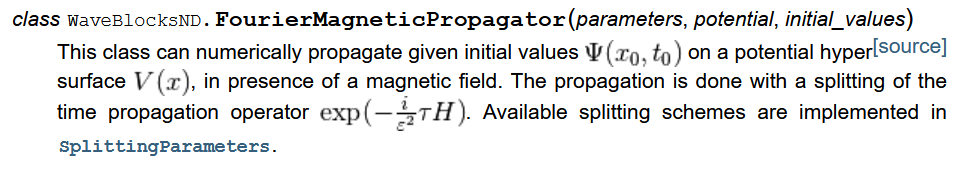
\includegraphics[width = 0.9\textwidth]{graphics/doc_fmp.PNG}
  \caption{Documentation-Header of the FourierMagneticPropagator Class.}
  \label{fig:doc_fmp}
\end{figure}
The code of the \emph{postpropagate}-function is summarised in Algorithm \ref{alg:postpropagate} and can also be found in Appendix \ref{appendix:code}. It implements the propagator from equation \ref{alg:postpropagate} and is based on Algorithm 1 from \cite{paper_orvg}. Its header reads as portrayed in figure~\ref{fig:pp}.
\begin{figure}
  \centering
  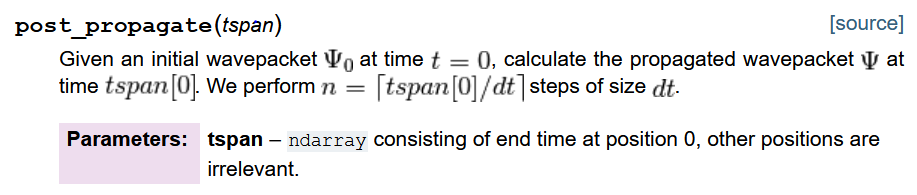
\includegraphics[width = 0.9 \textwidth]{graphics/doc_postpropagate.PNG}
  \caption{Header of the postpropagate-function.}
  \label{fig:pp}
\end{figure}

The flow map $\rho$ from equation \ref{eq_rho} effectively acts as a rotation. These rotations could not directly be applied onto the potential $V$ or the wavefunction $\Psi$ but had to be realised via a rotation of the underlying grid $X$. More precisely, the operation $(\rho(R)A)(x) = A(R^{-1}x)$ requires us to first rotate the grid $X$ by $R^{-1}$ and then evaluate the quantity $A$ on the rotated grid. Because $X$ is a class member in WaveBlocksND, after the evaluation of $A$ on $R^{-1}\cdot X$ we need to reverse the above rotation to return to the original state. \newline
Because of the rotational invariance of the first term in equation \ref{eq:rotinv}, in the term $\Phi_{\rho(U(t_0 + Nh, t_i + jh))V}$ only the electric potential $\phi$ needs to be subjected to such a rotation.

\begin{algorithm}[h]
  \label{alg:postpropagate}
    \SetAlgoLined
    \caption{PostPropagate Function}
    \BlankLine

    \KwData{\emph{As arguments to the function:} class instance $self$; end time $t$.\newline \emph{As arguments to the class instance:} step width $dt$; meshgrid $X$; initial wave function $\Psi_0$; potential $V$; magnetic field $B$; number of components of the wavefunction $N$; quantisation parameter $\epsilon$; splitting method with coefficients $(a_i, b_i)_{i = 1}^n$; end time of simulation $T$; dimension $d$; frequency of writing to disk $w_n$.}
    \KwResult{ Computes wavepacket at time $t$ and saves it to class member. \textbf{Returns:} End time $t$.}

    define stepwidth: $n_{steps}$ = $\lceil t / dt \rceil $\;
    define time grids: $t_a = t_0$, $t_b = t_0$ \;
    calculate flow map $R = U(t_0 + N\cdot dt, t_0)$ \;
    rotate the grid by $R^T$ \;
    evaluate initial data on rotated grid and save to wavefunction $\Psi$\;
    rotate grid back \;

    \For{j = 0 to nsteps}{
      \For{i = 0 to dim(a)}{
        potential propagator $\Phi_V = \Phi_{B} \cdot \Phi_{\phi}:$ \\{
          \Indp calculate magnetic field propagator $\Phi_{B} = \exp(-i \langle x, (\int_{t_a}^{t_a + a_i \cdot dt} B^2(s) ds)x \rangle)$ \;
          apply propagator to $\Psi$ \;
          rotate grid by $R^T$ \;
          calculate electric and external potential propagator $\Phi_{\phi} = \exp(-i \int_{t_a}^{t_a + a_i \cdot dt} (\phi(x,s) + V_{ext}) ds)$ \;
          apply propagator to $\Psi$ on rotated grid \;
          rotate grid back \;
        }
        calculate flow map $R = R\cdot U^{-1}(t_b + b_i \cdot dt, t_b)$ \;
        kinetic propagator $\Phi_{-\Delta}$: \\
        {
          \Indp Fast-Fourier-Transform $\Psi$ to Fourier space \;
          calculate the kinetic propagator $Phi_{-\Delta}$ \;
          apply propagator to $\mathcal{FFT}(\Psi)$ \;
          Inverse-FFT $\Psi$ to real space \;
        }
        update time grids: $t_a = t_a + a_i \cdot dt$, $t_b = t_b + b_i \cdot dt$ \;
      }
    }
    \Return{t}

\end{algorithm}


\section{Results}

//include convergence plots here

//also include wavefct plot and discuss similarities to paper

\section{Summary and Conclusion}

\begin{appendices}


\section{Code} \label{appendix:code}
    \lstdefinestyle{mystyle}{
    backgroundcolor=\color{backcolour},
    commentstyle=\color{codegreen},
    keywordstyle=\color{magenta},
    numberstyle=\tiny\color{codegray},
    stringstyle=\color{codepurple},
    basicstyle=\ttfamily\footnotesize,
    breakatwhitespace=false,
    breaklines=true,
    captionpos=b,
    keepspaces=true,
    numbers=left,
    numbersep=5pt,
    showspaces=false,
    showstringspaces=false,
    showtabs=false,
    tabsize=2
}

\lstset{style=mystyle}

%%\inputminted{python}{../FourierMagneticPropagator.py}

%% make sure to refresh this at the end
\lstinputlisting[language=Python]{../FourierMagneticPropagator.py}

%%\begin{Verbatim}[commandchars=\\\{\}]
\PY{l+s+sa}{r}\PY{l+s+sd}{\PYZdq{}\PYZdq{}\PYZdq{}The WaveBlocks Project}

\PY{l+s+sd}{This file contains the Fourier Magnetic Propagator class. The wavefunction}
\PY{l+s+sd}{:math:`\PYZbs{}Psi` is propagated in time with a splitting of the}
\PY{l+s+sd}{exponential :math:`\PYZbs{}exp(\PYZhy{}\PYZbs{}frac\PYZob{}i\PYZcb{}\PYZob{}\PYZbs{}varepsilon\PYZca{}2\PYZcb{} \PYZbs{}tau H)`.}

\PY{l+s+sd}{@author: R. Bourquin}
\PY{l+s+sd}{@copyright: Copyright (C) 2012, 2016 R. Bourquin}
\PY{l+s+sd}{@license: Modified BSD License}
\PY{l+s+sd}{\PYZdq{}\PYZdq{}\PYZdq{}}

\PY{k+kn}{from} \PY{n+nn}{numpy} \PY{k+kn}{import} \PY{n}{array}\PY{p}{,} \PY{n}{complexfloating}\PY{p}{,} \PY{n}{dot}\PY{p}{,} \PY{n}{exp}\PY{p}{,} \PY{n}{eye}\PY{p}{,} \PY{n}{zeros}\PY{p}{,} \PY{n}{shape}
\PY{k+kn}{from} \PY{n+nn}{numpy.fft} \PY{k+kn}{import} \PY{n}{fftn}\PY{p}{,} \PY{n}{ifftn}
\PY{k+kn}{from} \PY{n+nn}{scipy.linalg} \PY{k+kn}{import} \PY{n}{expm}

\PY{k+kn}{from} \PY{n+nn}{WaveBlocksND.BlockFactory} \PY{k+kn}{import} \PY{n}{BlockFactory}
\PY{k+kn}{from} \PY{n+nn}{WaveBlocksND.Propagator} \PY{k+kn}{import} \PY{n}{Propagator}
\PY{k+kn}{from} \PY{n+nn}{WaveBlocksND.KineticOperator} \PY{k+kn}{import} \PY{n}{KineticOperator}
\PY{k+kn}{from} \PY{n+nn}{WaveBlocksND.MagneticField} \PY{k+kn}{import} \PY{n}{MagneticField}
\PY{k+kn}{from} \PY{n+nn}{WaveBlocksND.SplittingParameters} \PY{k+kn}{import} \PY{n}{SplittingParameters}

\PY{n}{\PYZus{}\PYZus{}all\PYZus{}\PYZus{}} \PY{o}{=} \PY{p}{[}\PY{l+s+s2}{\PYZdq{}}\PY{l+s+s2}{FourierMagneticPropagator}\PY{l+s+s2}{\PYZdq{}}\PY{p}{]}


\PY{k}{class} \PY{n+nc}{FourierMagneticPropagator}\PY{p}{(}\PY{n}{Propagator}\PY{p}{,} \PY{n}{SplittingParameters}\PY{p}{)}\PY{p}{:}
    \PY{l+s+sa}{r}\PY{l+s+sd}{\PYZdq{}\PYZdq{}\PYZdq{}This class can numerically propagate given initial values :math:`\PYZbs{}Psi(x\PYZus{}0, t\PYZus{}0)` on}
\PY{l+s+sd}{    a potential hyper surface :math:`V(x)`, in presence of a magnetic field. The propagation is done with a splitting}
\PY{l+s+sd}{    of the time propagation operator :math:`\PYZbs{}exp(\PYZhy{}\PYZbs{}frac\PYZob{}i\PYZcb{}\PYZob{}\PYZbs{}varepsilon\PYZca{}2\PYZcb{} \PYZbs{}tau H)`.}
\PY{l+s+sd}{    Available splitting schemes are implemented in :py:class:`SplittingParameters`.}
\PY{l+s+sd}{    \PYZdq{}\PYZdq{}\PYZdq{}}

    \PY{k}{def} \PY{n+nf+fm}{\PYZus{}\PYZus{}init\PYZus{}\PYZus{}}\PY{p}{(}\PY{n+nb+bp}{self}\PY{p}{,} \PY{n}{parameters}\PY{p}{,} \PY{n}{potential}\PY{p}{,} \PY{n}{initial\PYZus{}values}\PY{p}{)}\PY{p}{:}
        \PY{l+s+sa}{r}\PY{l+s+sd}{\PYZdq{}\PYZdq{}\PYZdq{}Initialize a new :py:class:`FourierMagneticPropagator` instance. Precalculate the}
\PY{l+s+sd}{        the kinetic operator :math:`T\PYZus{}e` and the potential operator :math:`V\PYZus{}e`}
\PY{l+s+sd}{        used for time propagation.}

\PY{l+s+sd}{        :param parameters: The set of simulation parameters. It must contain at least}
\PY{l+s+sd}{                           the semi\PYZhy{}classical parameter :math:`\PYZbs{}varepsilon` and the}
\PY{l+s+sd}{                           time step size :math:`\PYZbs{}tau`.}
\PY{l+s+sd}{        :param potential: The potential :math:`V(x)` governing the time evolution.}
\PY{l+s+sd}{        :type potential: A :py:class:`MatrixPotential` instance.}
\PY{l+s+sd}{        :param initial\PYZus{}values: The initial values :math:`\PYZbs{}Psi(\PYZbs{}Gamma, t\PYZus{}0)` given}
\PY{l+s+sd}{                               in the canonical basis.}
\PY{l+s+sd}{        :type initial\PYZus{}values: A :py:class:`WaveFunction` instance.}

\PY{l+s+sd}{        :raise: :py:class:`ValueError` If the number of components of :math:`\PYZbs{}Psi` does not match the}
\PY{l+s+sd}{                           number of energy surfaces :math:`\PYZbs{}lambda\PYZus{}i(x)` of the potential.}

\PY{l+s+sd}{        :raise: :py:class:`ValueError` If the number of components of :math:`\PYZbs{}Psi` does not match the dimension of the magnetic field :math:`\PYZbs{}vec\PYZob{}B\PYZcb{}(x)`.}

\PY{l+s+sd}{        :raise: :py:class:`ValueError` If the dimensions of the splitting scheme parameters :math:`a` and :math:`b` are not equal.}
\PY{l+s+sd}{        \PYZdq{}\PYZdq{}\PYZdq{}}
        \PY{c+c1}{\PYZsh{} The embedded \PYZsq{}MatrixPotential\PYZsq{} instance representing the potential \PYZsq{}V\PYZsq{}.}
        \PY{n+nb+bp}{self}\PY{o}{.}\PY{n}{\PYZus{}potential} \PY{o}{=} \PY{n}{potential}

        \PY{c+c1}{\PYZsh{} The initial values of the components \PYZsq{}\PYZbs{}psi\PYZus{}i\PYZsq{} sampled at the given grid.}
        \PY{n+nb+bp}{self}\PY{o}{.}\PY{n}{\PYZus{}psi} \PY{o}{=} \PY{n}{initial\PYZus{}values}

        \PY{k}{if} \PY{n+nb+bp}{self}\PY{o}{.}\PY{n}{\PYZus{}potential}\PY{o}{.}\PY{n}{get\PYZus{}number\PYZus{}components}\PY{p}{(}\PY{p}{)} \PY{o}{!=} \PY{n+nb+bp}{self}\PY{o}{.}\PY{n}{\PYZus{}psi}\PY{o}{.}\PY{n}{get\PYZus{}number\PYZus{}components}\PY{p}{(}\PY{p}{)}\PY{p}{:}
            \PY{k}{raise} \PY{n+ne}{ValueError}\PY{p}{(}\PY{l+s+s2}{\PYZdq{}}\PY{l+s+s2}{Potential dimension and number of components do not match.}\PY{l+s+s2}{\PYZdq{}}\PY{p}{)}

        \PY{c+c1}{\PYZsh{} The time step size.}
        \PY{n+nb+bp}{self}\PY{o}{.}\PY{n}{\PYZus{}dt} \PY{o}{=} \PY{n}{parameters}\PY{p}{[}\PY{l+s+s2}{\PYZdq{}}\PY{l+s+s2}{dt}\PY{l+s+s2}{\PYZdq{}}\PY{p}{]}

        \PY{c+c1}{\PYZsh{} Final time.}
        \PY{n+nb+bp}{self}\PY{o}{.}\PY{n}{\PYZus{}T} \PY{o}{=} \PY{n}{parameters}\PY{p}{[}\PY{l+s+s2}{\PYZdq{}}\PY{l+s+s2}{T}\PY{l+s+s2}{\PYZdq{}}\PY{p}{]}

        \PY{c+c1}{\PYZsh{} The model parameter \PYZsq{}\PYZbs{}varepsilon\PYZsq{}.}
        \PY{n+nb+bp}{self}\PY{o}{.}\PY{n}{\PYZus{}eps} \PY{o}{=} \PY{n}{parameters}\PY{p}{[}\PY{l+s+s2}{\PYZdq{}}\PY{l+s+s2}{eps}\PY{l+s+s2}{\PYZdq{}}\PY{p}{]}

        \PY{c+c1}{\PYZsh{} Spacial dimension d}
        \PY{n+nb+bp}{self}\PY{o}{.}\PY{n}{\PYZus{}dimension} \PY{o}{=} \PY{n}{parameters}\PY{p}{[}\PY{l+s+s2}{\PYZdq{}}\PY{l+s+s2}{dimension}\PY{l+s+s2}{\PYZdq{}}\PY{p}{]}

        \PY{c+c1}{\PYZsh{} The position space grid nodes \PYZsq{}\PYZbs{}Gamma\PYZsq{}.}
        \PY{n+nb+bp}{self}\PY{o}{.}\PY{n}{\PYZus{}grid} \PY{o}{=} \PY{n}{initial\PYZus{}values}\PY{o}{.}\PY{n}{get\PYZus{}grid}\PY{p}{(}\PY{p}{)}

        \PY{c+c1}{\PYZsh{} The kinetic operator \PYZsq{}T\PYZsq{} defined in momentum space.}
        \PY{n+nb+bp}{self}\PY{o}{.}\PY{n}{\PYZus{}KO} \PY{o}{=} \PY{n}{KineticOperator}\PY{p}{(}\PY{n+nb+bp}{self}\PY{o}{.}\PY{n}{\PYZus{}grid}\PY{p}{,} \PY{n+nb+bp}{self}\PY{o}{.}\PY{n}{\PYZus{}eps}\PY{p}{)}

        \PY{c+c1}{\PYZsh{} Exponential \PYZsq{}\PYZbs{}exp(\PYZhy{}i/2*eps\PYZca{}2*dt*T)\PYZsq{} used in the Strang splitting.}
        \PY{c+c1}{\PYZsh{} not used}
        \PY{n+nb+bp}{self}\PY{o}{.}\PY{n}{\PYZus{}KO}\PY{o}{.}\PY{n}{calculate\PYZus{}exponential}\PY{p}{(}\PY{o}{\PYZhy{}}\PY{l+m+mf}{0.5j} \PY{o}{*} \PY{n+nb+bp}{self}\PY{o}{.}\PY{n}{\PYZus{}dt} \PY{o}{*} \PY{n+nb+bp}{self}\PY{o}{.}\PY{n}{\PYZus{}eps}\PY{o}{*}\PY{o}{*}\PY{l+m+mi}{2}\PY{p}{)}
        \PY{n+nb+bp}{self}\PY{o}{.}\PY{n}{\PYZus{}TE} \PY{o}{=} \PY{n+nb+bp}{self}\PY{o}{.}\PY{n}{\PYZus{}KO}\PY{o}{.}\PY{n}{evaluate\PYZus{}exponential\PYZus{}at}\PY{p}{(}\PY{p}{)}

        \PY{c+c1}{\PYZsh{} Exponential \PYZsq{}\PYZbs{}exp(\PYZhy{}i/eps\PYZca{}2*dt*V)\PYZsq{} used in the Strang splitting.}
        \PY{c+c1}{\PYZsh{} not used}
        \PY{n+nb+bp}{self}\PY{o}{.}\PY{n}{\PYZus{}potential}\PY{o}{.}\PY{n}{calculate\PYZus{}exponential}\PY{p}{(}\PY{o}{\PYZhy{}}\PY{l+m+mf}{0.5j} \PY{o}{*} \PY{n+nb+bp}{self}\PY{o}{.}\PY{n}{\PYZus{}dt} \PY{o}{/} \PY{n+nb+bp}{self}\PY{o}{.}\PY{n}{\PYZus{}eps}\PY{o}{*}\PY{o}{*}\PY{l+m+mi}{2}\PY{p}{)}
        \PY{n}{VE} \PY{o}{=} \PY{n+nb+bp}{self}\PY{o}{.}\PY{n}{\PYZus{}potential}\PY{o}{.}\PY{n}{evaluate\PYZus{}exponential\PYZus{}at}\PY{p}{(}\PY{n+nb+bp}{self}\PY{o}{.}\PY{n}{\PYZus{}grid}\PY{p}{)}
        \PY{n+nb+bp}{self}\PY{o}{.}\PY{n}{\PYZus{}VE} \PY{o}{=} \PY{n+nb}{tuple}\PY{p}{(}\PY{p}{[}\PY{n}{ve}\PY{o}{.}\PY{n}{reshape}\PY{p}{(}\PY{n+nb+bp}{self}\PY{o}{.}\PY{n}{\PYZus{}grid}\PY{o}{.}\PY{n}{get\PYZus{}number\PYZus{}nodes}\PY{p}{(}\PY{p}{)}\PY{p}{)} \PY{k}{for} \PY{n}{ve} \PY{o+ow}{in} \PY{n}{VE}\PY{p}{]}\PY{p}{)}

        \PY{c+c1}{\PYZsh{} The magnetic field}
        \PY{n+nb+bp}{self}\PY{o}{.}\PY{n}{\PYZus{}B} \PY{o}{=} \PY{n}{MagneticField}\PY{p}{(}\PY{n}{parameters}\PY{p}{[}\PY{l+s+s2}{\PYZdq{}}\PY{l+s+s2}{B}\PY{l+s+s2}{\PYZdq{}}\PY{p}{]}\PY{p}{)}
        \PY{c+c1}{\PYZsh{} check if magnetic field and potential are of same dimension}
        \PY{k}{if} \PY{n+nb+bp}{self}\PY{o}{.}\PY{n}{\PYZus{}B}\PY{o}{.}\PY{n}{get\PYZus{}dimension}\PY{p}{(}\PY{p}{)} \PY{o}{!=} \PY{n+nb+bp}{self}\PY{o}{.}\PY{n}{\PYZus{}dimension}\PY{p}{:}
            \PY{k}{raise} \PY{n+ne}{ValueError}\PY{p}{(}\PY{l+s+s2}{\PYZdq{}}\PY{l+s+s2}{Spacial dimension of potential and magnetic field must be the same}\PY{l+s+s2}{\PYZdq{}}\PY{p}{)}

        \PY{c+c1}{\PYZsh{}precalculate the splitting needed}
        \PY{n+nb+bp}{self}\PY{o}{.}\PY{n}{\PYZus{}a}\PY{p}{,} \PY{n+nb+bp}{self}\PY{o}{.}\PY{n}{\PYZus{}b} \PY{o}{=} \PY{n+nb+bp}{self}\PY{o}{.}\PY{n}{build}\PY{p}{(}\PY{n}{parameters}\PY{p}{[}\PY{l+s+s2}{\PYZdq{}}\PY{l+s+s2}{splitting\PYZus{}method}\PY{l+s+s2}{\PYZdq{}}\PY{p}{]}\PY{p}{)}
        \PY{k}{if} \PY{n}{shape}\PY{p}{(}\PY{n+nb+bp}{self}\PY{o}{.}\PY{n}{\PYZus{}a}\PY{p}{)} \PY{o}{!=} \PY{n}{shape}\PY{p}{(}\PY{n+nb+bp}{self}\PY{o}{.}\PY{n}{\PYZus{}b}\PY{p}{)}\PY{p}{:}
            \PY{k}{raise} \PY{n+ne}{ValueError}\PY{p}{(}\PY{l+s+s2}{\PYZdq{}}\PY{l+s+s2}{Splitting scheme shapes must be the same}\PY{l+s+s2}{\PYZdq{}}\PY{p}{)}

        \PY{c+c1}{\PYZsh{} Get inital data as function}
        \PY{n}{packet\PYZus{}descr} \PY{o}{=} \PY{n}{parameters}\PY{p}{[}\PY{l+s+s2}{\PYZdq{}}\PY{l+s+s2}{initvals}\PY{l+s+s2}{\PYZdq{}}\PY{p}{]}\PY{p}{[}\PY{l+m+mi}{0}\PY{p}{]}
        \PY{n+nb+bp}{self}\PY{o}{.}\PY{n}{\PYZus{}initalpacket} \PY{o}{=} \PY{n}{BlockFactory}\PY{p}{(}\PY{p}{)}\PY{o}{.}\PY{n}{create\PYZus{}wavepacket}\PY{p}{(}\PY{n}{packet\PYZus{}descr}\PY{p}{)}


    \PY{c+c1}{\PYZsh{} TODO: Consider removing this, duplicate}
    \PY{k}{def} \PY{n+nf}{get\PYZus{}number\PYZus{}components}\PY{p}{(}\PY{n+nb+bp}{self}\PY{p}{)}\PY{p}{:}
        \PY{l+s+sa}{r}\PY{l+s+sd}{\PYZdq{}\PYZdq{}\PYZdq{}Get the number :math:`N` of components of :math:`\PYZbs{}Psi`.}

\PY{l+s+sd}{        :return: The number :math:`N`.}
\PY{l+s+sd}{        \PYZdq{}\PYZdq{}\PYZdq{}}
        \PY{k}{return} \PY{n+nb+bp}{self}\PY{o}{.}\PY{n}{\PYZus{}potential}\PY{o}{.}\PY{n}{get\PYZus{}number\PYZus{}components}\PY{p}{(}\PY{p}{)}


    \PY{k}{def} \PY{n+nf}{get\PYZus{}wavefunction}\PY{p}{(}\PY{n+nb+bp}{self}\PY{p}{)}\PY{p}{:}
        \PY{l+s+sa}{r}\PY{l+s+sd}{\PYZdq{}\PYZdq{}\PYZdq{}Get the wavefunction that stores the current data :math:`\PYZbs{}Psi(\PYZbs{}Gamma)`.}

\PY{l+s+sd}{        :return: The :py:class:`WaveFunction` instance.}
\PY{l+s+sd}{        \PYZdq{}\PYZdq{}\PYZdq{}}
        \PY{k}{return} \PY{n+nb+bp}{self}\PY{o}{.}\PY{n}{\PYZus{}psi}


    \PY{k}{def} \PY{n+nf}{get\PYZus{}operators}\PY{p}{(}\PY{n+nb+bp}{self}\PY{p}{)}\PY{p}{:}
        \PY{l+s+sa}{r}\PY{l+s+sd}{\PYZdq{}\PYZdq{}\PYZdq{}Get the kinetic and potential operators :math:`T(\PYZbs{}Omega)` and :math:`V(\PYZbs{}Gamma)`.}

\PY{l+s+sd}{        :return: A tuple :math:`(T, V)` containing two ``ndarrays``.}
\PY{l+s+sd}{        \PYZdq{}\PYZdq{}\PYZdq{}}
        \PY{c+c1}{\PYZsh{} TODO: What kind of object exactly do we want to return?}
        \PY{n+nb+bp}{self}\PY{o}{.}\PY{n}{\PYZus{}KO}\PY{o}{.}\PY{n}{calculate\PYZus{}operator}\PY{p}{(}\PY{p}{)}
        \PY{n}{T} \PY{o}{=} \PY{n+nb+bp}{self}\PY{o}{.}\PY{n}{\PYZus{}KO}\PY{o}{.}\PY{n}{evaluate\PYZus{}at}\PY{p}{(}\PY{p}{)}
        \PY{n}{V} \PY{o}{=} \PY{n+nb+bp}{self}\PY{o}{.}\PY{n}{\PYZus{}potential}\PY{o}{.}\PY{n}{evaluate\PYZus{}at}\PY{p}{(}\PY{n+nb+bp}{self}\PY{o}{.}\PY{n}{\PYZus{}grid}\PY{p}{)}
        \PY{n}{V} \PY{o}{=} \PY{n+nb}{tuple}\PY{p}{(}\PY{p}{[}\PY{n}{v}\PY{o}{.}\PY{n}{reshape}\PY{p}{(}\PY{n+nb+bp}{self}\PY{o}{.}\PY{n}{\PYZus{}grid}\PY{o}{.}\PY{n}{get\PYZus{}number\PYZus{}nodes}\PY{p}{(}\PY{p}{)}\PY{p}{)} \PY{k}{for} \PY{n}{v} \PY{o+ow}{in} \PY{n}{V}\PY{p}{]}\PY{p}{)}
        \PY{k}{return} \PY{p}{(}\PY{n}{T}\PY{p}{,} \PY{n}{V}\PY{p}{)}


    \PY{n+nd}{@staticmethod}
    \PY{k}{def} \PY{n+nf}{\PYZus{}Magnus\PYZus{}CF4}\PY{p}{(}\PY{n}{tspan}\PY{p}{,} \PY{n}{B}\PY{p}{,} \PY{n}{N}\PY{p}{,} \PY{o}{*}\PY{n}{args}\PY{p}{)}\PY{p}{:}
        \PY{l+s+sa}{r}\PY{l+s+sd}{\PYZdq{}\PYZdq{}\PYZdq{}Returns the  Fourth Order Magnus integrator :math:`\PYZbs{}Omega(A)` according to [\PYZsh{}]\PYZus{}.}

\PY{l+s+sd}{        :param tspan: Full timespan of expansion.}

\PY{l+s+sd}{        :param B: Magnetic field matrix :math:`B(t) = (B\PYZus{}\PYZob{}j,k\PYZcb{}(t))\PYZus{}\PYZob{}1 \PYZbs{}leq j, k \PYZbs{}leq d\PYZcb{}`.}

\PY{l+s+sd}{        :param N: Number of timesteps for the expansion.}

\PY{l+s+sd}{        :param *args: Additional arguments for the magnetic field :math:`B(t, *args)`}

\PY{l+s+sd}{        .. [\PYZsh{}] S. Blanes and P.C. Moan. \PYZdq{}Fourth\PYZhy{} and sixth\PYZhy{}order commutator\PYZhy{}free Magnus integrators for linear and non\PYZhy{}linear dynamical systems\PYZdq{}. Applied Numerical Mathematics, 56(12):1519 \PYZhy{} 1537, 2006.}
\PY{l+s+sd}{        \PYZdq{}\PYZdq{}\PYZdq{}}
        \PY{c+c1}{\PYZsh{} Magnus constants}
        \PY{n}{c1} \PY{o}{=} \PY{l+m+mf}{0.5}\PY{o}{*}\PY{p}{(}\PY{l+m+mf}{1.0} \PY{o}{\PYZhy{}} \PY{l+m+mf}{0.5773502691896258}\PY{p}{)}
        \PY{n}{c2} \PY{o}{=} \PY{l+m+mf}{0.5}\PY{o}{*}\PY{p}{(}\PY{l+m+mf}{1.0} \PY{o}{+} \PY{l+m+mf}{0.5773502691896258}\PY{p}{)}
        \PY{n}{a1} \PY{o}{=} \PY{l+m+mf}{0.5}\PY{o}{*}\PY{p}{(}\PY{l+m+mf}{0.5} \PY{o}{\PYZhy{}} \PY{l+m+mf}{0.5773502691896258}\PY{p}{)}
        \PY{n}{a2} \PY{o}{=} \PY{l+m+mf}{0.5}\PY{o}{*}\PY{p}{(}\PY{l+m+mf}{0.5} \PY{o}{+} \PY{l+m+mf}{0.5773502691896258}\PY{p}{)}

        \PY{n}{R} \PY{o}{=} \PY{l+m+mf}{1.}\PY{o}{*}\PY{n}{eye}\PY{p}{(} \PY{n+nb}{len}\PY{p}{(} \PY{n}{B}\PY{p}{(}\PY{l+m+mf}{1.}\PY{o}{*}\PY{n}{tspan}\PY{p}{[}\PY{l+m+mi}{0}\PY{p}{]}\PY{p}{,} \PY{o}{*}\PY{n}{args}\PY{p}{)} \PY{p}{)} \PY{p}{)}
        \PY{n}{h} \PY{o}{=} \PY{p}{(}\PY{n}{tspan}\PY{p}{[}\PY{l+m+mi}{1}\PY{p}{]}\PY{o}{\PYZhy{}}\PY{n}{tspan}\PY{p}{[}\PY{l+m+mi}{0}\PY{p}{]}\PY{p}{)} \PY{o}{/} \PY{p}{(}\PY{l+m+mf}{1.}\PY{o}{*}\PY{n}{N}\PY{p}{)}
        \PY{k}{for} \PY{n}{k} \PY{o+ow}{in} \PY{n+nb}{range}\PY{p}{(}\PY{n}{N}\PY{p}{)}\PY{p}{:}
            \PY{n}{t0} \PY{o}{=} \PY{n}{k}\PY{o}{*}\PY{n}{h} \PY{o}{+} \PY{n}{tspan}\PY{p}{[}\PY{l+m+mi}{0}\PY{p}{]}
            \PY{n}{t1} \PY{o}{=} \PY{n}{t0} \PY{o}{+} \PY{n}{c1}\PY{o}{*}\PY{n}{h}
            \PY{n}{t2} \PY{o}{=} \PY{n}{t0} \PY{o}{+} \PY{n}{c2}\PY{o}{*}\PY{n}{h}
            \PY{n}{B1} \PY{o}{=} \PY{n}{B}\PY{p}{(}\PY{n}{t1}\PY{p}{,} \PY{o}{*}\PY{n}{args}\PY{p}{)}
            \PY{n}{B2} \PY{o}{=} \PY{n}{B}\PY{p}{(}\PY{n}{t2}\PY{p}{,} \PY{o}{*}\PY{n}{args}\PY{p}{)}
            \PY{n}{R} \PY{o}{=} \PY{n}{dot}\PY{p}{(}\PY{n}{expm}\PY{p}{(}\PY{n}{a1}\PY{o}{*}\PY{n}{h}\PY{o}{*}\PY{n}{B1}\PY{o}{+}\PY{n}{a2}\PY{o}{*}\PY{n}{h}\PY{o}{*}\PY{n}{B2}\PY{p}{)}\PY{p}{,} \PY{n}{dot}\PY{p}{(}\PY{n}{expm}\PY{p}{(}\PY{n}{a2}\PY{o}{*}\PY{n}{h}\PY{o}{*}\PY{n}{B1}\PY{o}{+}\PY{n}{a1}\PY{o}{*}\PY{n}{h}\PY{o}{*}\PY{n}{B2}\PY{p}{)}\PY{p}{,} \PY{n}{R}\PY{p}{)}\PY{p}{)}

        \PY{k}{return} \PY{n}{R}


    \PY{k}{def} \PY{n+nf}{post\PYZus{}propagate}\PY{p}{(}\PY{n+nb+bp}{self}\PY{p}{,} \PY{n}{tspan}\PY{p}{)}\PY{p}{:}
        \PY{l+s+sa}{r}\PY{l+s+sd}{\PYZdq{}\PYZdq{}\PYZdq{}Given an initial wavepacket :math:`\PYZbs{}Psi\PYZus{}0` at time :math:`t=0`, calculate the propagated wavepacket :math:`\PYZbs{}Psi` at time :math:`tspan \PYZbs{}[ 0 \PYZbs{}]`. We perform :math:`n = \PYZbs{}lceil tspan\PYZbs{}[ 0 \PYZbs{}] /dt \PYZbs{}rceil` steps of size :math:`dt`.}

\PY{l+s+sd}{        :param tspan: :py class:`ndarray` consisting of end time at position 0, other positions are irrelevant.}
\PY{l+s+sd}{        \PYZdq{}\PYZdq{}\PYZdq{}}

        \PY{c+c1}{\PYZsh{} (ignoriere tspan[0])}
        \PY{n}{nsteps} \PY{o}{=} \PY{n+nb}{int}\PY{p}{(}\PY{n}{tspan}\PY{p}{[}\PY{l+m+mi}{0}\PY{p}{]} \PY{o}{/} \PY{n+nb+bp}{self}\PY{o}{.}\PY{n}{\PYZus{}dt} \PY{o}{+} \PY{l+m+mf}{0.5}\PY{p}{)}
        \PY{k}{print}\PY{p}{(}\PY{l+s+s2}{\PYZdq{}}\PY{l+s+s2}{Perform }\PY{l+s+s2}{\PYZdq{}} \PY{o}{+} \PY{n+nb}{str}\PY{p}{(}\PY{n}{nsteps}\PY{p}{)} \PY{o}{+} \PY{l+s+s2}{\PYZdq{}}\PY{l+s+s2}{ steps from t = 0.0 to t = }\PY{l+s+s2}{\PYZdq{}} \PY{o}{+} \PY{n+nb}{str}\PY{p}{(}\PY{n}{tspan}\PY{p}{[}\PY{l+m+mi}{0}\PY{p}{]}\PY{p}{)}\PY{p}{)}


        \PY{c+c1}{\PYZsh{} Magnetfeld Matrix B(t)}
        \PY{n}{B} \PY{o}{=} \PY{k}{lambda} \PY{n}{t}\PY{p}{:} \PY{n+nb+bp}{self}\PY{o}{.}\PY{n}{\PYZus{}B}\PY{p}{(}\PY{n}{t}\PY{p}{)}

        \PY{c+c1}{\PYZsh{}how many components does Psi have}
        \PY{n}{N} \PY{o}{=} \PY{n+nb+bp}{self}\PY{o}{.}\PY{n}{\PYZus{}psi}\PY{o}{.}\PY{n}{get\PYZus{}number\PYZus{}components}\PY{p}{(}\PY{p}{)}

        \PY{c+c1}{\PYZsh{}start time t\PYZus{}0 = 0?}
        \PY{n}{t0} \PY{o}{=} \PY{l+m+mi}{0}
        \PY{n}{t\PYZus{}a} \PY{o}{=} \PY{n}{t0}
        \PY{n}{t\PYZus{}b} \PY{o}{=} \PY{n}{t0}

        \PY{c+c1}{\PYZsh{}calculate R = U(t0 + N*h, t0)}
        \PY{c+c1}{\PYZsh{}Use N = n\PYZus{}steps to account for large time difference}
        \PY{n}{t\PYZus{}interval} \PY{o}{=} \PY{n}{array}\PY{p}{(}\PY{p}{[}\PY{n}{t0}\PY{p}{,} \PY{n}{tspan}\PY{p}{[}\PY{l+m+mi}{0}\PY{p}{]}\PY{p}{]}\PY{p}{)}
        \PY{n}{R} \PY{o}{=} \PY{n}{FourierMagneticPropagator}\PY{o}{.}\PY{n}{\PYZus{}Magnus\PYZus{}CF4}\PY{p}{(}\PY{n}{t\PYZus{}interval}\PY{p}{,} \PY{n}{B}\PY{p}{,} \PY{n}{nsteps}\PY{p}{)}

        \PY{c+c1}{\PYZsh{} rotate the grid by the transpose of R}
        \PY{n+nb+bp}{self}\PY{o}{.}\PY{n}{\PYZus{}grid}\PY{o}{.}\PY{n}{rotate}\PY{p}{(}\PY{n}{R}\PY{o}{.}\PY{n}{T}\PY{p}{)}

        \PY{c+c1}{\PYZsh{} Compute rotated initial data}
        \PY{n}{X} \PY{o}{=} \PY{n+nb+bp}{self}\PY{o}{.}\PY{n}{\PYZus{}grid}\PY{o}{.}\PY{n}{get\PYZus{}nodes}\PY{p}{(}\PY{n}{flat}\PY{o}{=}\PY{n+nb+bp}{True}\PY{p}{)}
        \PY{n}{values} \PY{o}{=} \PY{n+nb+bp}{self}\PY{o}{.}\PY{n}{\PYZus{}initalpacket}\PY{o}{.}\PY{n}{evaluate\PYZus{}at}\PY{p}{(}\PY{n}{X}\PY{p}{,} \PY{n}{prefactor}\PY{o}{=}\PY{n+nb+bp}{True}\PY{p}{)}
        \PY{n}{values} \PY{o}{=} \PY{n+nb}{tuple}\PY{p}{(}\PY{p}{[}\PY{n}{val}\PY{o}{.}\PY{n}{reshape}\PY{p}{(}\PY{n+nb+bp}{self}\PY{o}{.}\PY{n}{\PYZus{}grid}\PY{o}{.}\PY{n}{get\PYZus{}number\PYZus{}nodes}\PY{p}{(}\PY{p}{)}\PY{p}{)} \PY{k}{for} \PY{n}{val} \PY{o+ow}{in} \PY{n}{values}\PY{p}{]}\PY{p}{)}
        \PY{n+nb+bp}{self}\PY{o}{.}\PY{n}{\PYZus{}psi}\PY{o}{.}\PY{n}{set\PYZus{}values}\PY{p}{(}\PY{n}{values}\PY{p}{)}

        \PY{n+nb+bp}{self}\PY{o}{.}\PY{n}{\PYZus{}grid}\PY{o}{.}\PY{n}{rotate}\PY{p}{(}\PY{n}{R}\PY{p}{)}

        \PY{c+c1}{\PYZsh{}calculate the necessary timesteps}
        \PY{k}{for} \PY{n}{j} \PY{o+ow}{in} \PY{n+nb}{range}\PY{p}{(}\PY{n}{nsteps}\PY{p}{)}\PY{p}{:}
            \PY{k}{for} \PY{n}{i} \PY{o+ow}{in} \PY{n+nb}{range}\PY{p}{(}\PY{n+nb}{len}\PY{p}{(}\PY{n+nb+bp}{self}\PY{o}{.}\PY{n}{\PYZus{}a}\PY{p}{)}\PY{p}{)}\PY{p}{:}
                \PY{c+c1}{\PYZsh{} Integral \PYZhy{}\PYZbs{}int\PYZus{}\PYZob{}tspan[0]\PYZcb{}\PYZca{}\PYZob{}tspan[1]\PYZcb{}B\PYZca{}2(s)ds und zugehörige Propagation}
                \PY{c+c1}{\PYZsh{} (siehe Paper, Remark 3.1)}
                \PY{n}{minus\PYZus{}B\PYZus{}squared} \PY{o}{=} \PY{k}{lambda} \PY{n}{t}\PY{p}{:} \PY{p}{(}\PY{o}{\PYZhy{}}\PY{l+m+mf}{1.0}\PY{p}{)} \PY{o}{*} \PY{n}{dot}\PY{p}{(}\PY{n}{B}\PY{p}{(}\PY{n}{t}\PY{p}{)}\PY{p}{,} \PY{n}{B}\PY{p}{(}\PY{n}{t}\PY{p}{)}\PY{p}{)}
                \PY{n}{A} \PY{o}{=} \PY{l+m+mf}{1.0} \PY{o}{/} \PY{l+m+mf}{8.0} \PY{o}{*} \PY{n}{MagneticField}\PY{o}{.}\PY{n}{matrix\PYZus{}quad}\PY{p}{(}\PY{n}{minus\PYZus{}B\PYZus{}squared}\PY{p}{,} \PY{n}{t\PYZus{}a}\PY{p}{,} \PY{n}{t\PYZus{}a} \PY{o}{+} \PY{n+nb+bp}{self}\PY{o}{.}\PY{n}{\PYZus{}a}\PY{p}{[}\PY{n}{i}\PY{p}{]}\PY{o}{*}\PY{n+nb+bp}{self}\PY{o}{.}\PY{n}{\PYZus{}dt}\PY{p}{)}

                \PY{n}{X} \PY{o}{=} \PY{n+nb+bp}{self}\PY{o}{.}\PY{n}{\PYZus{}grid}\PY{o}{.}\PY{n}{get\PYZus{}nodes}\PY{p}{(}\PY{n}{flat}\PY{o}{=}\PY{n+nb+bp}{True}\PY{p}{)}
                \PY{n}{VB} \PY{o}{=} \PY{n+nb}{sum}\PY{p}{(}\PY{n}{X} \PY{o}{*} \PY{n}{dot}\PY{p}{(}\PY{n}{A}\PY{p}{,} \PY{n}{X}\PY{p}{)}\PY{p}{)}
                \PY{n}{VB} \PY{o}{=} \PY{n}{VB}\PY{o}{.}\PY{n}{reshape}\PY{p}{(}\PY{n+nb+bp}{self}\PY{o}{.}\PY{n}{\PYZus{}grid}\PY{o}{.}\PY{n}{get\PYZus{}number\PYZus{}nodes}\PY{p}{(}\PY{p}{)}\PY{p}{)}
                \PY{n}{prop} \PY{o}{=} \PY{n}{exp}\PY{p}{(}\PY{o}{\PYZhy{}}\PY{l+m+mf}{1.0j} \PY{o}{/} \PY{n+nb+bp}{self}\PY{o}{.}\PY{n}{\PYZus{}eps}\PY{o}{*}\PY{o}{*}\PY{l+m+mi}{2} \PY{o}{*} \PY{n}{VB}\PY{p}{)} \PY{c+c1}{\PYZsh{} ev. \PYZhy{}0.5j durch \PYZhy{}1j ersetzen...}

                \PY{n}{values} \PY{o}{=} \PY{n+nb+bp}{self}\PY{o}{.}\PY{n}{\PYZus{}psi}\PY{o}{.}\PY{n}{get\PYZus{}values}\PY{p}{(}\PY{p}{)}
                \PY{n}{values} \PY{o}{=} \PY{p}{[}\PY{n}{prop} \PY{o}{*} \PY{n}{component} \PY{k}{for} \PY{n}{component} \PY{o+ow}{in} \PY{n}{values}\PY{p}{]}

                \PY{n+nb+bp}{self}\PY{o}{.}\PY{n}{\PYZus{}potential}\PY{o}{.}\PY{n}{calculate\PYZus{}exponential}\PY{p}{(}\PY{o}{\PYZhy{}}\PY{l+m+mf}{1.0j} \PY{o}{*}  \PY{n+nb+bp}{self}\PY{o}{.}\PY{n}{\PYZus{}a}\PY{p}{[}\PY{n}{i}\PY{p}{]}\PY{o}{*}\PY{n+nb+bp}{self}\PY{o}{.}\PY{n}{\PYZus{}dt} \PY{o}{/}\PY{n+nb+bp}{self}\PY{o}{.}\PY{n}{\PYZus{}eps}\PY{o}{*}\PY{o}{*}\PY{l+m+mi}{2}\PY{p}{)}

                \PY{n+nb+bp}{self}\PY{o}{.}\PY{n}{\PYZus{}grid}\PY{o}{.}\PY{n}{rotate}\PY{p}{(}\PY{n}{R}\PY{o}{.}\PY{n}{T}\PY{p}{)}
                \PY{n}{VE} \PY{o}{=} \PY{n+nb+bp}{self}\PY{o}{.}\PY{n}{\PYZus{}potential}\PY{o}{.}\PY{n}{evaluate\PYZus{}exponential\PYZus{}at}\PY{p}{(}\PY{n+nb+bp}{self}\PY{o}{.}\PY{n}{\PYZus{}grid}\PY{p}{)}
                \PY{n+nb+bp}{self}\PY{o}{.}\PY{n}{\PYZus{}VE} \PY{o}{=} \PY{n+nb}{tuple}\PY{p}{(}\PY{p}{[}\PY{n}{ve}\PY{o}{.}\PY{n}{reshape}\PY{p}{(}\PY{n+nb+bp}{self}\PY{o}{.}\PY{n}{\PYZus{}grid}\PY{o}{.}\PY{n}{get\PYZus{}number\PYZus{}nodes}\PY{p}{(}\PY{p}{)}\PY{p}{)} \PY{k}{for} \PY{n}{ve} \PY{o+ow}{in} \PY{n}{VE}\PY{p}{]}\PY{p}{)}

                \PY{c+c1}{\PYZsh{}apply it}
                \PY{n}{values} \PY{o}{=} \PY{p}{[}\PY{n+nb+bp}{self}\PY{o}{.}\PY{n}{\PYZus{}VE} \PY{o}{*} \PY{n}{component} \PY{k}{for} \PY{n}{component} \PY{o+ow}{in} \PY{n}{values}\PY{p}{]}
                \PY{n+nb+bp}{self}\PY{o}{.}\PY{n}{\PYZus{}grid}\PY{o}{.}\PY{n}{rotate}\PY{p}{(}\PY{n}{R}\PY{p}{)}

                \PY{n}{t\PYZus{}interval}\PY{p}{[}\PY{l+m+mi}{0}\PY{p}{]} \PY{o}{=} \PY{n}{t\PYZus{}b}
                \PY{n}{t\PYZus{}interval}\PY{p}{[}\PY{l+m+mi}{1}\PY{p}{]} \PY{o}{=} \PY{n}{t\PYZus{}b} \PY{o}{+} \PY{n+nb+bp}{self}\PY{o}{.}\PY{n}{\PYZus{}b}\PY{p}{[}\PY{n}{i}\PY{p}{]}\PY{o}{*}\PY{n+nb+bp}{self}\PY{o}{.}\PY{n}{\PYZus{}dt}

                \PY{n}{U} \PY{o}{=} \PY{p}{(}\PY{n}{FourierMagneticPropagator}\PY{o}{.}\PY{n}{\PYZus{}Magnus\PYZus{}CF4}\PY{p}{(}\PY{n}{t\PYZus{}interval}\PY{p}{,} \PY{n}{B}\PY{p}{,} \PY{l+m+mi}{1}\PY{p}{)}\PY{p}{)}\PY{o}{.}\PY{n}{T}
                \PY{n}{R} \PY{o}{=} \PY{n}{dot}\PY{p}{(}\PY{n}{R} \PY{p}{,} \PY{n}{U}\PY{p}{)}
                \PY{k}{if}\PY{p}{(}\PY{n}{R}\PY{o}{.}\PY{n}{shape} \PY{o}{!=} \PY{n}{U}\PY{o}{.}\PY{n}{shape}\PY{p}{)}\PY{p}{:}
                    \PY{k}{raise} \PY{n+ne}{ValueError}\PY{p}{(}\PY{l+s+s2}{\PYZdq{}}\PY{l+s+s2}{Shapes of R and U do not match}\PY{l+s+s2}{\PYZdq{}}\PY{p}{)}

                \PY{c+c1}{\PYZsh{}check for obsolete splitting steps}
                \PY{k}{if}\PY{p}{(}\PY{n+nb+bp}{self}\PY{o}{.}\PY{n}{\PYZus{}b}\PY{p}{[}\PY{n}{i}\PY{p}{]} \PY{o}{!=} \PY{l+m+mi}{0}\PY{p}{)}\PY{p}{:}
                    \PY{n}{values} \PY{o}{=} \PY{p}{[}\PY{n}{fftn}\PY{p}{(}\PY{n}{component}\PY{p}{)} \PY{k}{for} \PY{n}{component} \PY{o+ow}{in} \PY{n}{values}\PY{p}{]}

                    \PY{c+c1}{\PYZsh{} Apply the kinetic operator}
                    \PY{n+nb+bp}{self}\PY{o}{.}\PY{n}{\PYZus{}KO} \PY{o}{=} \PY{n}{KineticOperator}\PY{p}{(}\PY{n+nb+bp}{self}\PY{o}{.}\PY{n}{\PYZus{}grid}\PY{p}{,} \PY{n+nb+bp}{self}\PY{o}{.}\PY{n}{\PYZus{}eps}\PY{p}{)}
                    \PY{n+nb+bp}{self}\PY{o}{.}\PY{n}{\PYZus{}KO}\PY{o}{.}\PY{n}{calculate\PYZus{}exponential}\PY{p}{(}\PY{o}{\PYZhy{}}\PY{l+m+mf}{0.5j} \PY{o}{*} \PY{n+nb+bp}{self}\PY{o}{.}\PY{n}{\PYZus{}eps}\PY{o}{*}\PY{o}{*}\PY{l+m+mi}{2} \PY{o}{*} \PY{n+nb+bp}{self}\PY{o}{.}\PY{n}{\PYZus{}b}\PY{p}{[}\PY{n}{i}\PY{p}{]}\PY{o}{*}\PY{n+nb+bp}{self}\PY{o}{.}\PY{n}{\PYZus{}dt}\PY{p}{)}

                    \PY{n}{TE} \PY{o}{=} \PY{n+nb+bp}{self}\PY{o}{.}\PY{n}{\PYZus{}KO}\PY{o}{.}\PY{n}{evaluate\PYZus{}exponential\PYZus{}at}\PY{p}{(}\PY{p}{)}
                    \PY{n}{values} \PY{o}{=} \PY{p}{[}\PY{n}{TE} \PY{o}{*} \PY{n}{component} \PY{k}{for} \PY{n}{component} \PY{o+ow}{in} \PY{n}{values}\PY{p}{]}

                    \PY{c+c1}{\PYZsh{} Go back to real space}
                    \PY{n}{values} \PY{o}{=} \PY{p}{[}\PY{n}{ifftn}\PY{p}{(}\PY{n}{component}\PY{p}{)} \PY{k}{for} \PY{n}{component} \PY{o+ow}{in} \PY{n}{values}\PY{p}{]}

                \PY{c+c1}{\PYZsh{}Apply}
                \PY{n+nb+bp}{self}\PY{o}{.}\PY{n}{\PYZus{}psi}\PY{o}{.}\PY{n}{set\PYZus{}values}\PY{p}{(}\PY{n}{values}\PY{p}{)}

                \PY{c+c1}{\PYZsh{}update t\PYZus{}a and t\PYZus{}b}
                \PY{n}{t\PYZus{}a} \PY{o}{=} \PY{n}{t\PYZus{}a} \PY{o}{+} \PY{n+nb+bp}{self}\PY{o}{.}\PY{n}{\PYZus{}a}\PY{p}{[}\PY{n}{i}\PY{p}{]}\PY{o}{*}\PY{n+nb+bp}{self}\PY{o}{.}\PY{n}{\PYZus{}dt}
                \PY{n}{t\PYZus{}b} \PY{o}{=} \PY{n}{t\PYZus{}b} \PY{o}{+} \PY{n+nb+bp}{self}\PY{o}{.}\PY{n}{\PYZus{}b}\PY{p}{[}\PY{n}{i}\PY{p}{]}\PY{o}{*}\PY{n+nb+bp}{self}\PY{o}{.}\PY{n}{\PYZus{}dt}

        \PY{k}{return} \PY{n}{tspan}\PY{p}{[}\PY{l+m+mi}{0}\PY{p}{]}


    \PY{k}{def} \PY{n+nf}{propagate}\PY{p}{(}\PY{n+nb+bp}{self}\PY{p}{,} \PY{n}{tspan}\PY{p}{)}\PY{p}{:}
        \PY{l+s+sa}{r}\PY{l+s+sd}{\PYZdq{}\PYZdq{}\PYZdq{}This method does nothing.}
\PY{l+s+sd}{        \PYZdq{}\PYZdq{}\PYZdq{}}
\end{Verbatim}


\end{appendices}


\begin{thebibliography}{9}
\bibitem{paper_orvg}
  V. Gradinaru and O. Rietmann.
  \emph{A High-Order Integrator for the
          Schr{\"o}dinger Equation with Time-Dependent,
          Homogeneous Magnetic Field}.
  Unpublished article, ETH Z{\"u}rich, submitted for publication, 2020.
\bibitem{simon_reed}
  B. Simon and M. Reed.
  \emph{Fourier Analysis, Self-Adjointness, Volume 2} of \emph{Methods of Modern Mathematical Physics}.
  Academic Press, Boston, 1975.
\bibitem{magnus_integrators}
  S. Blanes and P.C. Moan.
  \emph{Fourth- and sixth-order commutator-free Magnus integrators for linear and non-linear dynamical systems}.
  Applied Numerical Mathematics, 56(12):1519 - 1537, 2006.
\bibitem{waveblocksnd}
  R. Bourquin and V. Gradinaru.
  \emph{{WaveBlocks}: Reusable building blocks for simulations with semiclassical wavepackets},
  GitHub, URL: \url{https://github.com/WaveBlocks/WaveBlocksND},
  2010 - 2016.

\end{thebibliography}

\end{document}
